%%%%%%%%%%%%%%%%%%%%%%%%%%%%%%%%%%%%%%%%%%%%%%%%%%%%%%%%%%%%%%%%%%%%%%%%%%%%%%%
%%                                                                           %%
%%   Dr Derek Harter                                                         %%
%%   Profesor, Department of Computer Science                                %% 
%%   Texas A&M University - Commerce, USA                                    %%
%%                                                                           %%
%%%%%%%%%%%%%%%%%%%%%%%%%%%%%%%%%%%%%%%%%%%%%%%%%%%%%%%%%%%%%%%%%%%%%%%%%%%%%%%
%%%%     SETTING STARTS - DO NOT CHANGE Unless your TeX setting require so   %%
%%%%%%%%%%%%%%%%%%%%%%%%%%%%%%%%%%%%%%%%%%%%%%%%%%%%%%%%%%%%%%%%%%%%%%%%%%%%%%%
%%----------------------------------------------------------------------------------
% DO NOT Change this. It is the required setting letterpaper page, 11pt, onside print, book style
%%----------------------------------------------------------------------------------
\documentclass[letterpaper,11pt,oneside]{book}

%%-------------------------------------
%% Page margin settings - % half inch margin all sides (recommended)
%%-------------------------------------
\usepackage[margin=1.2in]{geometry} 

%%-------------------------------------
%% Font settings - % CM San or Ariel (recommended)
%%-------------------------------------
% Switch the following two line off: to revert back to default LaTex font (NOT recommended)
\usepackage{amsfonts}
\renewcommand*\familydefault{\sfdefault}

%%-------------------------------------
%% Math/Definition/Theorem/Algorithm packages settings 
%%-------------------------------------
\usepackage[cmex10]{amsmath}
\usepackage{amssymb}
\usepackage{amsthm}
\newtheorem{mydef}{Definition}
\newtheorem{mytherm}{Theorem}

%%-------------------------------------
%% Algorithms/Code Listing environment settings  - 
%% Please do not change these settings
%%-------------------------------------
\usepackage{algorithm}
\usepackage{algpseudocode}
\renewcommand{\algorithmicrequire}{\textbf{Input:}}
\renewcommand{\algorithmicensure}{\textbf{Output:}}
\usepackage[utf8]{inputenc}
\usepackage{listings}
\usepackage{xcolor}
\definecolor{codegreen}{rgb}{0,0.6,0.1}
\definecolor{codegray}{rgb}{0.5,0.5,0.5}
\definecolor{codeblue}{rgb}{0.10,0.00,1.00}
\definecolor{codepurple}{rgb}{0.58,0,0.82}
\definecolor{backcolour}{rgb}{1.0,1.0,1.0}

\lstdefinestyle{mystyle}{
    backgroundcolor=\color{backcolour},   
    commentstyle=\color{codegreen},
    keywordstyle=\color{codeblue},
    numberstyle=\tiny\color{codegray},
    stringstyle=\color{codepurple},
    basicstyle=\ttfamily\footnotesize,
    breakatwhitespace=false,         
    breaklines=true,                 
    captionpos=b,                        
    keepspaces=true,                 
    numbers=left,                    
    numbersep=5pt,                  
    showspaces=false,                
    showstringspaces=false,
    showtabs=false,                  
    tabsize=2,
    frame=none
}
\lstset{style=mystyle}

%%-------------------------------------
%% Graphics/Figures environment settings
%%-------------------------------------
\usepackage{graphicx}
\usepackage{subfigure}
\usepackage{caption}
\usepackage{lipsum}

%%-------------------------------------
%% Table environment settings
%%-------------------------------------
\usepackage{multirow}
\usepackage{rotating}
\usepackage{makecell}
\usepackage{booktabs}
%\usepackage{longtable,booktabs}

%%-------------------------------------
%% List of Abbreviations settings
%%-------------------------------------
\usepackage{enumitem}
\newlist{abbrv}{itemize}{1}
\setlist[abbrv,1]{label=,labelwidth=1in,align=parleft,itemsep=0.1\baselineskip,leftmargin=!}

%%-------------------------------------
%% Bibliography/References settings   - Harvard Style was used in this report
%%-------------------------------------
\usepackage[hidelinks]{hyperref}
\usepackage[comma,authoryear]{natbib}
\renewcommand{\bibname}{References} % DO NOT remove or switch of 

%%-------------------------------------
%% Appendix settings     
%%-------------------------------------
\usepackage[toc]{appendix}
%%%%%%%%%%%%%%%%%%%%%%%%%%%%%%%%%%%%%%%%%%%%%%%%%%%%%%%%%%%%%%%%%%%%%%%%%%%%%%%%%%%%%%%
%%%%                     SETTING ENDS                                            %%%%%%
%%%%%%%%%%%%%%%%%%%%%%%%%%%%%%%%%%%%%%%%%%%%%%%%%%%%%%%%%%%%%%%%%%%%%%%%%%%%%%%%%%%%%%%
\begin{document}

    \captionsetup[figure]{margin=1.5cm,font=small,name={Figure},labelsep=colon}
    \captionsetup[table]{margin=1.5cm,font=small,name={Table},labelsep=colon}
    \SetLipsumDefault{1}
    
    \frontmatter
    
    \begin{titlepage}      
        \begin{center}
            
\includegraphics[width=3cm]{figures/tamuc-logo.png}\\[0.5cm]
            {\LARGE Texas A\&M University - Commerce\\[0.5cm]
            Department of Computer Science}\\[2cm]
			%{\color{blue} \rule{\textwidth}{1pt}}
			
			% -------------------------------
			% You need to edit some details here
			% -------------------------------  
            \linespread{1.2}\huge {
                %%%%%%%%%%%%%%%%%%%%%%%%%%%%
                %TODO: 1 TITLE of Your PROJECT 
                %%%%%%%%%%%%%%%%%%%%%%%%%%%%
                % chnage the following line                
                Comparative Analysis of Autoencoders and Standard Deep Networks for MNIST Classification
            
            }
            \linespread{1}~\\[2cm]
			%{\color{blue} \rule{\textwidth}{1pt}}
            {\Large 
                %%%%%%%%%%%%%%%%%%%%%%%%%%%%
                %TODO: 2 YOUR NAME
                %%%%%%%%%%%%%%%%%%%%%%%%%%%%             
                % chnage the following line
                Bharath Muthuswamy Paran
                % change end             
            }\\[1cm] 
            

            {\large 
                %%%%%%%%%%%%%%%%%%%%%%%%%%%%
                %TODO: 3 YOUR NAME Supervisor's name(s)
                %%%%%%%%%%%%%%%%%%%%%%%%%%%%             
                % change the following line                
                \emph{Supervisor:} Derek Harter, Ph.D.}\\[1cm] % if applicable
            
    		% PLEASE DO NOT CHANGE THIS TEXT %
            \large A report submitted in partial fulfilment of the requirements of\\Texas A\&M University - Commerce for the degree of\\ Master of Science in \textit{Computer Science}\\[0.3cm] 
            \vfill
            
            
            \today % Please update this date you can use \date{April 2020} for fixed date
        \end{center}
    \end{titlepage}
    
    
    % -------------------------------------------------------------------
    % Declaration
    % -------------------------------------------------------------------
    \newpage
    \thispagestyle{empty}
    \chapter*{\Large Declaration}
    % PLEASE CHANGE THIS TEXT EXCEPT YOUR NAME%
    % -------------------------------
    %TODO: PLEASE ONLY UPDATE HERE -- PLEASE WRITE YOUR NAME %    
    % ------------------------------- 
    I,
    %%%%%%%%%%%%%%%%%%%%%%%
     Bharath Muthuswamy Paran, % Mandatory part
    %%%%%%%%%%%%%%%%%%%%%%%
    of the Department of Computer Science, Texas A\&M University - Commerce, confirm that this is my own work and figures, tables, equations, code snippets, artworks, and illustrations in this report are original and have not been taken from any other person's work, except where the works of others have been explicitly acknowledged, quoted, and referenced. I understand that if failing to do so will be considered a case of plagiarism. Plagiarism is a form of academic misconduct and will be penalised accordingly. \\
    
    %% Please delete as appropriate. 
    \noindent
    %%%%%%%%%%%%%%%%%%%%%%%%%%%%%%%%%%%%%%%%%%%%%%% 
    %TODO 1 Consent for example copy -  we will use 
    I give consent to a copy of my report being shared with future students as an exemplar. \\
    
    \noindent
    %%%%%%%%%%%%%%%%%%%%%%%%%%%%%%%%%%%%%%%%%%%%%%% 
    %TODO 2 Consent to let the report to use use by library for public use
    I give consent for my work to be made available more widely to members of TAMUC and public with interest in teaching, learning and research. 
    %%%%%%%%%%%%%%%%%%%%%%%%%%%%%%%%%%%%%%%%%%%%%%%
    ~\\[1cm]
    \begin{flushright}
	%------------------------------ 
	% change the following line
    %TODO: PLEASE UPDATE  Your Name  -------------------------------%
	Bharath Muthuswamy Paran % Please change it to your name
    
    \today
    \end{flushright}

     
    % -------------------------------------------------------------------
    % Abstract and Acknowledgement
    % -------------------------------------------------------------------
    
    %Two resources useful for abstract writing.
% Guidance of how to write an abstract/summary provided by Nature: https://cbs.umn.edu/sites/cbs.umn.edu/files/public/downloads/Annotated_Nature_abstract.pdf %https://writingcenter.gmu.edu/guides/writing-an-abstract
\chapter*{\center \Large  Abstract}
%%%%%%%%%%%%%%%%%%%%%%%%%%%%%%%%%%%%%%
% Replace all text with your text
%%%%%%%%%%%%%%%%%%%%%%%%%%%%%%%%%%%

In order to enchance MNIST classification this research focused to conduct an in-depth 
comparative analysis between two powerful architectures: the Denoising Autoencoder (DAE) and 
the Convolutional Neural Network (CNN). Both models are well-regarded for their distinct 
capabilities — DAE excels in unsupervised learning and feature extraction, while CNN is 
tailored for image-based tasks, particularly  classification. Motivated by the imperative to 
enhance the robustness of MNIST digit classification, this study navigates through the 
architectures of DAE and CNN, analyzing their impact on classification accuracy and noise 
resilience. The research extends beyond traditional performance metrics, delving into the 
interpretability of learned representations and assessing the models' ability to handle noisy 
input data. The research problem centers on deciphering how these architectures influence MNIST 
classification under varying levels of noise, providing insights into their respective 
strengths and limitations.  By addressing this research problem, the study aims to contribute 
to the advancement of image classification techniques, offering nuanced guidance on selecting 
models for MNIST classification tasks, especially in scenarios with noisy input data. The 
significance of this research lies in its potential to improve the resilience of classification 
models to real-world noise, thereby enhancing their applicability in practical settings. The 
findings are expected to benefit practitioners and researchers alike, guiding them in the 
selection and optimization of models for noise-affected MNIST classification scenarios.


~\\[1cm]
\noindent % Provide your key words
\textbf{Keywords:} Deep Learning, Denoising Autoencoder,
Convolutional Neural Networks, Classification, Accuracy.
    % -------------------------------------------------------------------
	% Acknowledgement
	% -------------------------------------------------------------------
   
    \chapter*{\center \Large  Acknowledgements}
%%%% Update with your text %%%%%%%%%%%%%%%
An acknowledgements section is optional. You may like to acknowledge the support and help of your supervisor(s), friends, or any other person(s), department(s), institute(s), etc. If you have been provided specific facility from department/school acknowledged so.  

   
    
    % -------------------------------------------------------------------
    % Contents, list of figures, list of tables
    % -------------------------------------------------------------------
    
    \tableofcontents
    \listoffigures
    \listoftables
    \chapter*{List of Abbreviations}
\chaptermark{List of Abbreviations}
%%%%%%%%%%%%%%%%%%%%%%%%%%%%%%%%%%%
%%  Enter your list of Abbreviation and Symbols in this file
%%%%%%%%%%%%%%%%%%%%%%%%%%%%%%%%%%%
\begin{abbrv}
    
    \item[SMPCS]			School of Mathematical, Physical and Computational Sciences
    
\end{abbrv}
 %  Enter your list of Abbreviation and Symbols in this file
    
    %%%%%%%%%%%%%%%%%%%%%%%%%%%%%%%%%%%%%%%%%%%%%%%%%%%%%%%%%%%%%%%%%%%%%%%%
    %%                                                                    %%  
    %%  Main chapters and sections of your project                        %%  
    %%  Everything from here on needs updates in your own words and works %%
    %%                                                                    %%
    %%%%%%%%%%%%%%%%%%%%%%%%%%%%%%%%%%%%%%%%%%%%%%%%%%%%%%%%%%%%%%%%%%%%%%%%
    \mainmatter
    % Read for preparation of document in LaTex 
    % Lamport, L. (1986), LATEX: A Document Preparation System, Addison-Wesley.
    
    \chapter{Introduction}
\label{ch:into} % This how you label a chapter and the key (e.g., ch:into) will be used to refer this chapter ``Introduction'' later in the report. 
% the key ``ch:into'' can be used with command \ref{ch:intor} to refere this Chapter.
The realm of image classification, a complex perceptual task involving the categorization of objects from images, has witnessed significant advancements over the past decade. Referred to as the process of categorizing objects, image classification relies on the sophisticated analysis of multispectral data, utilizing the underlying multispectral pattern of each pixel as a quantitative basis for classification \cite{lillesand2015remote}. Notably, there has been a remarkable improvement in classification accuracy, reflecting the evolution of image classification models. In recent times, these models are increasingly applied across diverse fields, showcasing their versatility. Applications range from tasks such as handwritten digit recognition \cite{ahlawat2020improved} and  Vehicle detection and classification \cite{tsai2018vehicle}, deep learning approach to pneumonia classification \cite{stephen2019efficient}, and military object detection \cite{janakiramaiah2023military}. The existing models are broadly categorized into unsupervised and supervised modes, reflecting the diverse approaches employed in addressing the intricate challenges of image classification.



%%%%%%%%%%%%%%%%%%%%%%%%%%%%%%%%%%%%%%%%%%%%%%%%%%%%%%%%%%%%%%%%%%%%%%%%%%%%%%%%%%%
\section{Background}
\label{sec:into_back}
The motivation behind this project stems from the imperative to enhance the robustness of MNIST digit classification, a task with applications ranging from digit recognition in postal services to the development of advanced optical character recognition systems. 

% \textbf{Cautions:} Do not say you choose this project because of your interest, or your supervisor proposed/suggested this project, or you were assigned this project as your final year project. This all may be true, but it is not meant to be written here.

%%%%%%%%%%%%%%%%%%%%%%%%%%%%%%%%%%%%%%%%%%%%%%%%%%%%%%%%%%%%%%%%%%%%%%%%%%%%%%%%%%%
\section{Problem statement}
\label{sec:intro_prob_art}
This section describes the investigated problem in detail. You can also have a separate chapter on ``Problem articulation.''  For some projects, you may have a section like ``Research question(s)'' or ``Research Hypothesis'' instead of a section on ``Problem statement.'

%%%%%%%%%%%%%%%%%%%%%%%%%%%%%%%%%%%%%%%%%%%%%%%%%%%%%%%%%%%%%%%%%%%%%%%%%%%%%%%%%%%
\section{Aims and objectives}
\label{sec:intro_aims_obj}
Describe the ``aims and objectives'' of your project. 

\textbf{Aims:} The aims tell a read what you want/hope to achieve at the end of the project. The  aims define your intent/purpose in general terms.  

\textbf{Objectives:} The objectives are a set of tasks you would perform in order to achieve the defined aims. The objective statements have to be specific and measurable through the results and outcome of the project.



%%%%%%%%%%%%%%%%%%%%%%%%%%%%%%%%%%%%%%%%%%%%%%%%%%%%%%%%%%%%%%%%%%%%%%%%%%%%%%%%%%%
\section{Solution approach}
\label{sec:intro_sol} % label of Org section
Briefly describe the solution approach and the methodology applied in solving the set aims and objectives.

Depending on the project, you may like to alter the ``heading'' of this section. Check with you supervisor. Also, check what subsection or any other section that can be added in or removed from this template.

\subsection{A subsection 1}
\label{sec:intro_some_sub1}
You may or may not need subsections here. Depending on your project's needs, add two or more subsection(s). A section takes at least two subsections. 

\subsection{A subsection 2}
\label{sec:intro_some_sub2}
Depending on your project's needs, add more section(s) and subsection(s).

\subsubsection{A subsection 1 of a subsection}
\label{sec:intro_some_subsub1}
The command \textbackslash subsubsection\{\} creates a paragraph heading in \LaTeX.

\subsubsection{A subsection 2 of a subsection}
\label{sec:intro_some_subsub2}
Write your text here...

%%%%%%%%%%%%%%%%%%%%%%%%%%%%%%%%%%%%%%%%%%%%%%%%%%%%%%%%%%%%%%%%%%%%%%%%%%%%%%%%%%%
\section{Summary of contributions and achievements} %  use this section 
\label{sec:intro_sum_results} % label of summary of results
Describe clearly what you have done/created/achieved and what the major results and their implications are. 


%%%%%%%%%%%%%%%%%%%%%%%%%%%%%%%%%%%%%%%%%%%%%%%%%%%%%%%%%%%%%%%%%%%%%%%%%%%%%%%%%%%
\section{Organization of the report} %  use this section
\label{sec:intro_org} % label of Org section
Describe the outline of the rest of the report here. Let the reader know what to expect ahead in the report. Describe how you have organized your report. 

\textbf{Example: how to refer a chapter, section, subsection}. This report is organised into seven chapters. Chapter~\ref{ch:lit_rev} details the literature review of this project. In Section~\ref{ch:method}...  % and so on.

\textbf{Note:}  Take care of the word like ``Chapter,'' ``Section,'' ``Figure'' etc. before the \LaTeX command \textbackslash ref\{\}. Otherwise, a  sentence will be confusing. For example, In \ref{ch:lit_rev} literature review is described. In this sentence, the word ``Chapter'' is missing. Therefore, a reader would not know whether 2 is for a Chapter or a Section or a Figure.


    \chapter{Literature Review}
\label{ch:lit_rev} %Label of the chapter lit rev. The key ``ch:lit_rev'' can be used with command \ref{ch:lit_rev} to refer this Chapter.


This section explores the existing existing body of knowledge surrounding the Comparative Analysis of Denoising Autoencoder (DAE) and Convolutional Neural Networks (CNN) for MNIST Classification. Recent advancements in deep machine learning have significantly improved feature learning in image processing tasks, particularly in image classification, making it imperative to explore and understand the capabilities and limitations of different models. Notably, Convolutional Neural Networks (CNNs) have emerged as powerful tools, showcasing superior performance in image classification tasks. However, the inherent challenge of noise in real-world data poses a significant constraint on the performance of deep neural networks, prompting the exploration of denoising techniques. The literature review will examine prior studies focusing on image denoising methods, including traditional approaches and those leveraging deep learning, with a specific emphasis on Denoising Autoencoders. Understanding the existing landscape is crucial for contextualizing the current research and identifying gaps that the Comparative Analysis seeks to address.

\section{Review of state-of-the-art}
The \citep{8078730} explores the application of deep learning, specifically Convolutional Neural Networks (CNNs), in image classification. The authors discuss various models commonly used in deep learning, such as Auto Encoder, sparse coding, Restricted Boltzmann Machine, Deep Belief Networks, and CNNs. They emphasize the effectiveness of CNNs in image classification, particularly showcasing their high performance. The study involves building a simple CNN for image classification, with experiments conducted on benchmark datasets like minist and cifar-10. The authors delve into the fundamental components of CNNs, including Convolutional layers, pooling layers, and fully-connected layers. The study focuses on learning rate strategies and optimization algorithms for solving optimal parameters in image classification. Different strategies are compared, demonstrating the impact on recognition rates during training and testing. 
The experimental results and 

The \citep{bajaj2020autoencoders} proposes an efficient image denoising technique using autoencoders based on deep learning models. The motivation behind image denoising is to eliminate noise from images, which can be caused by various factors such as defects in camera sensors, transmission in noisy channels, or faulty memory locations in hardware. The proposed model utilizes autoencoders, a type of artificial neural network, for image denoising. Autoencoders learn noise patterns from training images and attempt to eliminate noise from novel images. The proposed network architecture consists of convolutional denoising autoencoder (CDA) blocks, each containing internal layers like convolution, pooling, deconvolution, and upsampling. Skip connections are employed to enhance the model's ability to capture finer image details and facilitate backpropagation during training. The paper discusses related work, highlighting methods such as non-local means, Block Matching and 3D Matching (BM3D), and denoising autoencoders. STL-10 dataset for training and the SET5 standard image dataset for testing. Performance metrics, such as Peak Signal-to-Noise Ratio (PSNR) and Structural Similarity Index (SSIM), are used to evaluate the proposed model's effectiveness in comparison to baseline models. The results show that the proposed model outperforms Convolutional Denoising Deep Neural Network (CDDNN) and Residual Encoder Decoder with 30 layers (RED30) in terms of PSNR, indicating superior denoising capabilities.

\section{Convolutional Neural Networks}
CNNs are a variant of multi-layered neural networks designed for
processing two-dimensional data, particularly well-suited for classifying visual patterns like pixel images with minimal pre-processing.
Feature extraction from observed data occurs at each layer by 
applying digital filtering techniques, allowing information to propagate through multiple layers.

THe CNN architecture, introduced by LeCun et al. in 1998, are
applied to classify images and perceive visual patterns directly
from pixel images. Information propagation throughout multiple layers
enables feature extraction using digital filtering techniques.
CNNs perform two main processes: convolution and subsampling. 
The convolution involves applying a small-sized kernel over the input
feature map (IFM) to produce a convolved feature map (CFM). CFMs are
computed by applying the convolutional operation over the original
input image using a kernel, which represents weights and biases.
Weights are shared among positions, preserving spatial locality during
the convolution process. The subsampling simplifies the feature map 
gained from convolution by selecting significant features and 
discarding the rest. Max-pooling, a subsampling method used in 
experiments, involves taking the maximum value over non-overlapping
sub-regions.

\section{Denoising Auto-Encoder}
Denoising Autoencoder (DAE) is a specialized type of artificial neural network designed to clean up noisy or corrupted data. It belongs to the family of autoencoders, which are neural networks trained to learn efficient representations of input data. DAEs, in particular, excel in removing noise and capturing essential features from corrupted input.

The encoder is the first part of the DAE. Its role is to transform the input data into a compressed representation. This compressed representation should ideally retain the essential features of the input while filtering out noise.
One distinctive feature of DAE is the intentional introduction of noise into the input data. This could involve adding random variations or distortions to simulate real-world noise or corruption.The decoder is the second part of the DAE. It takes the compressed representation from the encoder and reconstructs the clean version of the original input data. The decoder's task is to recover the essential features and remove the injected noise.

% A possible section of you chapter
\section{Critique of the review} % Use this section title or choose a betterone
The literature review provides a comprehensive overview of the existing body of knowledge on the Comparative Analysis of Denoising Autoencoder (DAE) and Convolutional Neural Networks (CNN) for MNIST Classification. The review is structured logically, beginning with an introduction to the significance of the topic and progressing to a review of state-of-the-art research.

\begin{itemize}
    \item Clear Problem Statement: The literature review effectively establishes the problem by highlighting the challenges posed by noise in real-world data for deep neural networks. The motivation to explore denoising techniques is well justified in the context of advancements in deep machine learning and the superior performance of CNNs in image classification.

    \item Thorough State-of-the-Art Review: The review of state-of-the-art research is well-detailed, discussing relevant models in deep learning for image classification, such as Auto Encoder, sparse coding, Restricted Boltzmann Machine, Deep Belief Networks, and CNNs. The exploration of fundamental components of CNNs, learning rate strategies, and optimization algorithms adds depth to the understanding of the field.

    \item Comprehensive Denoising Technique Overview: The literature appropriately includes a discussion on denoising techniques, with a specific emphasis on the proposed model using autoencoders. The incorporation of related work, including traditional methods like non-local means and modern approaches like denoising autoencoders, enriches the background information.

    \item Methodology Explanation: The detailed description of the proposed image denoising technique using convolutional denoising autoencoder (CDA) blocks, skip connections, and performance metrics (PSNR and SSIM) adds transparency to the methodology.

    \item Effective Comparison of Models: The comparative analysis between the proposed model and existing models like Convolutional Denoising Deep Neural Network (CDDNN) and Residual Encoder Decoder with 30 layers (RED30) is valuable. The use of performance metrics provides a quantitative basis for comparison.

% Pleae use this section
\section{Summary} 

In this literature review, the Comparative Analysis of Denoising Autoencoder (DAE) and Convolutional Neural Networks (CNN) for MNIST Classification is explored within the context of recent advancements in deep machine learning. Convolutional Neural Networks (CNNs) have shown superior performance in image classification tasks, but the challenge of noise in real-world data necessitates the investigation of denoising techniques. The review critically examines prior studies on image denoising, with a specific focus on Denoising Autoencoders.

The state-of-the-art review discusses the application of CNNs in image classification, emphasizing their effectiveness. It covers various deep learning models, including Auto Encoder, sparse coding, Restricted Boltzmann Machine, and Deep Belief Networks, with experiments conducted on benchmark datasets. Another study proposes an image denoising technique using autoencoders, demonstrating its effectiveness through metrics like Peak Signal-to-Noise Ratio (PSNR) and Structural Similarity Index (SSIM). The proposed model outperforms existing models, showcasing superior denoising capabilities. The comprehensive overview of denoising techniques, methodology transparency, and effective comparison of models contribute to the overall strength of the literature review. This groundwork sets the stage for the Comparative Analysis, aiming to address gaps in understanding and provide insights into the capabilities and limitations of DAEs and CNNs for MNIST Classification.% https://guides.library.bloomu.edu/litreview
    % replace all text with your own text.
% in this template few examples are mention
\chapter{Methodology}
\label{ch:method} % Label for method chapter
\section{Convolutional Neural Networks}
CNNs are a variant of multi-layered neural networks designed for
processing two-dimensional data, particularly well-suited for classifying visual patterns like pixel images with minimal pre-processing.
Feature extraction from observed data occurs at each layer by 
applying digital filtering techniques, allowing information to propagate through multiple layers.

THe CNN architecture, introduced by LeCun et al. in 1998, are
applied to classify images and perceive visual patterns directly
from pixel images. Information propagation throughout multiple layers
enables feature extraction using digital filtering techniques.
CNNs perform two main processes: convolution and subsampling. 
The convolution involves applying a small-sized kernel over the input
feature map (IFM) to produce a convolved feature map (CFM). CFMs are
computed by applying the convolutional operation over the original
input image using a kernel, which represents weights and biases.
Weights are shared among positions, preserving spatial locality during
the convolution process. The subsampling simplifies the feature map 
gained from convolution by selecting significant features and 
discarding the rest. Max-pooling, a subsampling method used in 
experiments, involves taking the maximum value over non-overlapping
sub-regions.

\section{Denoising Auto-Encoder}
Denoising Autoencoder (DAE) is a specialized type of artificial neural network designed to clean up noisy or corrupted data. It belongs to the family of autoencoders, which are neural networks trained to learn efficient representations of input data. DAEs, in particular, excel in removing noise and capturing essential features from corrupted input.

The encoder is the first part of the DAE. Its role is to transform the input data into a compressed representation. This compressed representation should ideally retain the essential features of the input while filtering out noise.
One distinctive feature of DAE is the intentional introduction of noise into the input data. This could involve adding random variations or distortions to simulate real-world noise or corruption.The decoder is the second part of the DAE. It takes the compressed representation from the encoder and reconstructs the clean version of the original input data. The decoder's task is to recover the essential features and remove the injected noise.

\section{Examples of the sections of a methodology chapter}
A general report structure is summarised (suggested) in Table~\ref{tab:gen_template}. Table~\ref{tab:gen_template} describes that, in general, a typical report structure has three main parts: (1) front matter, (2) main text, and (3) end matter. %[\textbf{also notice that the preceding sentence is an example of a numbered list in a text body}]. 
The structure of the front matter and end matter will remain the same for all the undergraduate final year project report. However, the main text varies as per the project's needs.
\begin{table}[ht!]
    \centering
    \caption{Undergraduate report template structure}
    \label{tab:gen_template}
    \begin{tabular}{llll}     
        \toprule
        \multirow{7}{3cm}{Frontmatter} 
        & & Title Page & \\                  
        & & Abstract &    \\          
        & & Acknowledgements & \\                            
        & & Table of Contents &    \\                                
        & & List of Figures   &    \\                        
        & & List of Tables    &    \\                
        & & List of Abbreviations  &    \\                     
        & &   &    \\                        
        \multirow{7}{3cm}{Main text}
        & Chapter 1 & Introduction   &    \\                         
        & Chapter 2 & Literature Review   &    \\
        & Chapter 3 & Methodology   &    \\
        & Chapter 4 & Results    &    \\
        & Chapter 5 & Discussion and Analysis  &    \\
        & Chapter 6 & Conclusions and Future Work  &    \\        
        & Chapter 7 & Refection  &    \\          
        & &   &    \\                       
        \multirow{2}{3cm}{End matter}
        & & References  &    \\   
        & & Appendices (Optional)  &    \\ 
        & & Index (Optional)  &    \\ 
        \bottomrule
    \end{tabular}
\end{table}

\subsection{Example of a software/Web development main text structure}
\label{subsec:se_chpters}
Notice that the ``methodology'' Chapter of Software/Web development in Table~\ref{tab:soft_eng_temp} takes a standard software engineering paradigm (approach). Alternatively, these suggested sections can be the chapters of their own. Also, notice that ``Chapter 5'' in Table~\ref{tab:soft_eng_temp} is ``Testing and Validation'' which is different from the general report template mentioned in Table~\ref{tab:gen_template}. Check with your supervisor if in doubt.
\begin{table}[ht!]
    \centering
    \caption{Example of a software engineering-type report structure}
    \label{tab:soft_eng_temp}
    \begin{tabular}{lll}     
        \toprule                   
        Chapter 1 & Introduction   &    \\        
        Chapter 2 & Literature Review  &    \\                   
        Chapter 3 & Methodology   &    \\
        &               & Requirements specifications   \\
        &               & Analysis   \\
        &               & Design   \\
        &               & Implementations   \\
        Chapter 4 & Testing and Validation  &    \\
        Chapter 5 & Results and Discussion      &    \\
        Chapter 6 & Conclusions and Future Work  &    \\        
        Chapter 7 & Reflection  &    \\                          
        \bottomrule
    \end{tabular}
\end{table}

\subsection{Example of an algorithm analysis main text structure}
Some project might involve the implementation of a state-of-the-art algorithm and its performance analysis and comparison with other algorithms. In that case, the suggestion in Table~\ref{tab:algo_temp} may suit you the best. 
\begin{table}[ht!]
    \centering
    \caption{Example of an algorithm analysis type report structure}
    \label{tab:algo_temp}
    \begin{tabular}{lll}     
        \toprule                   
        Chapter 1 & Introduction  &    \\        
        Chapter 2 & Literature Review  &    \\                
        Chapter 3 & Methodology   &    \\
        &               & Algorithms descriptions  \\
        &               & Implementations   \\
        &               & Experiments design   \\
        Chapter 4 & Results       &  \\
        Chapter 5 & Discussion and Analysis  &    \\
        Chapter 6 & Conclusion and Future Work  &    \\        
        Chapter 7 & Reflection  &    \\          
        \bottomrule
    \end{tabular}
\end{table}

\subsection{Example of an application type main text structure}
If you are applying some algorithms/tools/technologies on some problems/datasets/etc., you may use the methodology section prescribed in Table~\ref{tab:app_temp}.  
\begin{table}[ht!]
    \centering
    \caption{Example of an application type report structure}
    \label{tab:app_temp}
    \begin{tabular}{lll}     
        \toprule                   
        Chapter 1 & Introduction  &    \\        
        Chapter 2 & Literature Review  &    \\                
        Chapter 3 & Methodology   &    \\
        &               & Problems (tasks) descriptions  \\
        &               & Algorithms/tools/technologies/etc. descriptions  \\        
        &               & Implementations   \\
        &               & Experiments design and setup   \\
        Chapter 4 & Results       &  \\
        Chapter 5 & Discussion and Analysis  &    \\
        Chapter 6 & Conclusion and Future Work  &    \\        
        Chapter 7 & Reflection  &    \\          
        \bottomrule
    \end{tabular}
\end{table}

\subsection{Example of a science lab-type main text structure}
If you are doing a science lab experiment type of project, you may use the  methodology section suggested in Table~\ref{tab:lab_temp}. In this kind of project, you may refer to the ``Methodology'' section as ``Materials and Methods.''
\begin{table}[ht!]
    \centering
    \caption{Example of a science lab experiment-type report structure}
    \label{tab:lab_temp}
    \begin{tabular}{lll}     
        \toprule                   
        Chapter 1 & Introduction  &    \\        
        Chapter 2 & Literature Review  &    \\                
        Chapter 3 & Materials and Methods   &    \\
        &               & Problems (tasks) description  \\
        &               & Materials \\        
        &               & Procedures  \\                
        &               & Implementations   \\
        &               & Experiment set-up   \\
        Chapter 4 & Results       &  \\
        Chapter 5 & Discussion and Analysis  &    \\
        Chapter 6 & Conclusion and Future Work  &    \\        
        Chapter 7 & Reflection  &    \\          
        \bottomrule
    \end{tabular}
\end{table}

\section{Example of an Equation in \LaTeX}
Eq.~\ref{eq:eq_example} [note that this is an example of an equation's in-text citation] is an example of an equation in \LaTeX. In Eq.~\eqref{eq:eq_example}, $ s $ is the mean of elements $ x_i \in \mathbf{x} $: 

\begin{equation}
\label{eq:eq_example} % label used to refer the eq in text
s = \frac{1}{N} \sum_{i = 1}^{N} x_i. 
\end{equation}

Have you noticed that all the variables of the equation are defined using the \textbf{in-text} maths command \$.\$, and Eq.~\eqref{eq:eq_example} is treated as a part of the sentence with proper punctuation? Always treat an equation or expression as a part of the sentence. 

\section{Example of a Figure in \LaTeX}
Figure~\ref{fig:chart_a} is an example of a figure in \LaTeX. For more details, check the link:

\href{https://en.wikibooks.org/wiki/LaTeX/Floats,_Figures_and_Captions}{wikibooks.org/wiki/LaTeX/Floats,\_Figures\_and\_Captions}.

\noindent
Keep your artwork (graphics, figures, illustrations) clean and readable. At least 300dpi is a good resolution of a PNG format artwork. However, an SVG format artwork saved as a PDF will produce the best quality graphics. There are numerous tools out there that can produce vector graphics and let you save that as an SVG file and/or as a PDF file. One example of such a tool is the ``Flow algorithm software''. Here is the link for that: \href{http://www.flowgorithm.org/download/}{flowgorithm.org}.
\begin{figure}[ht]
    \centering
    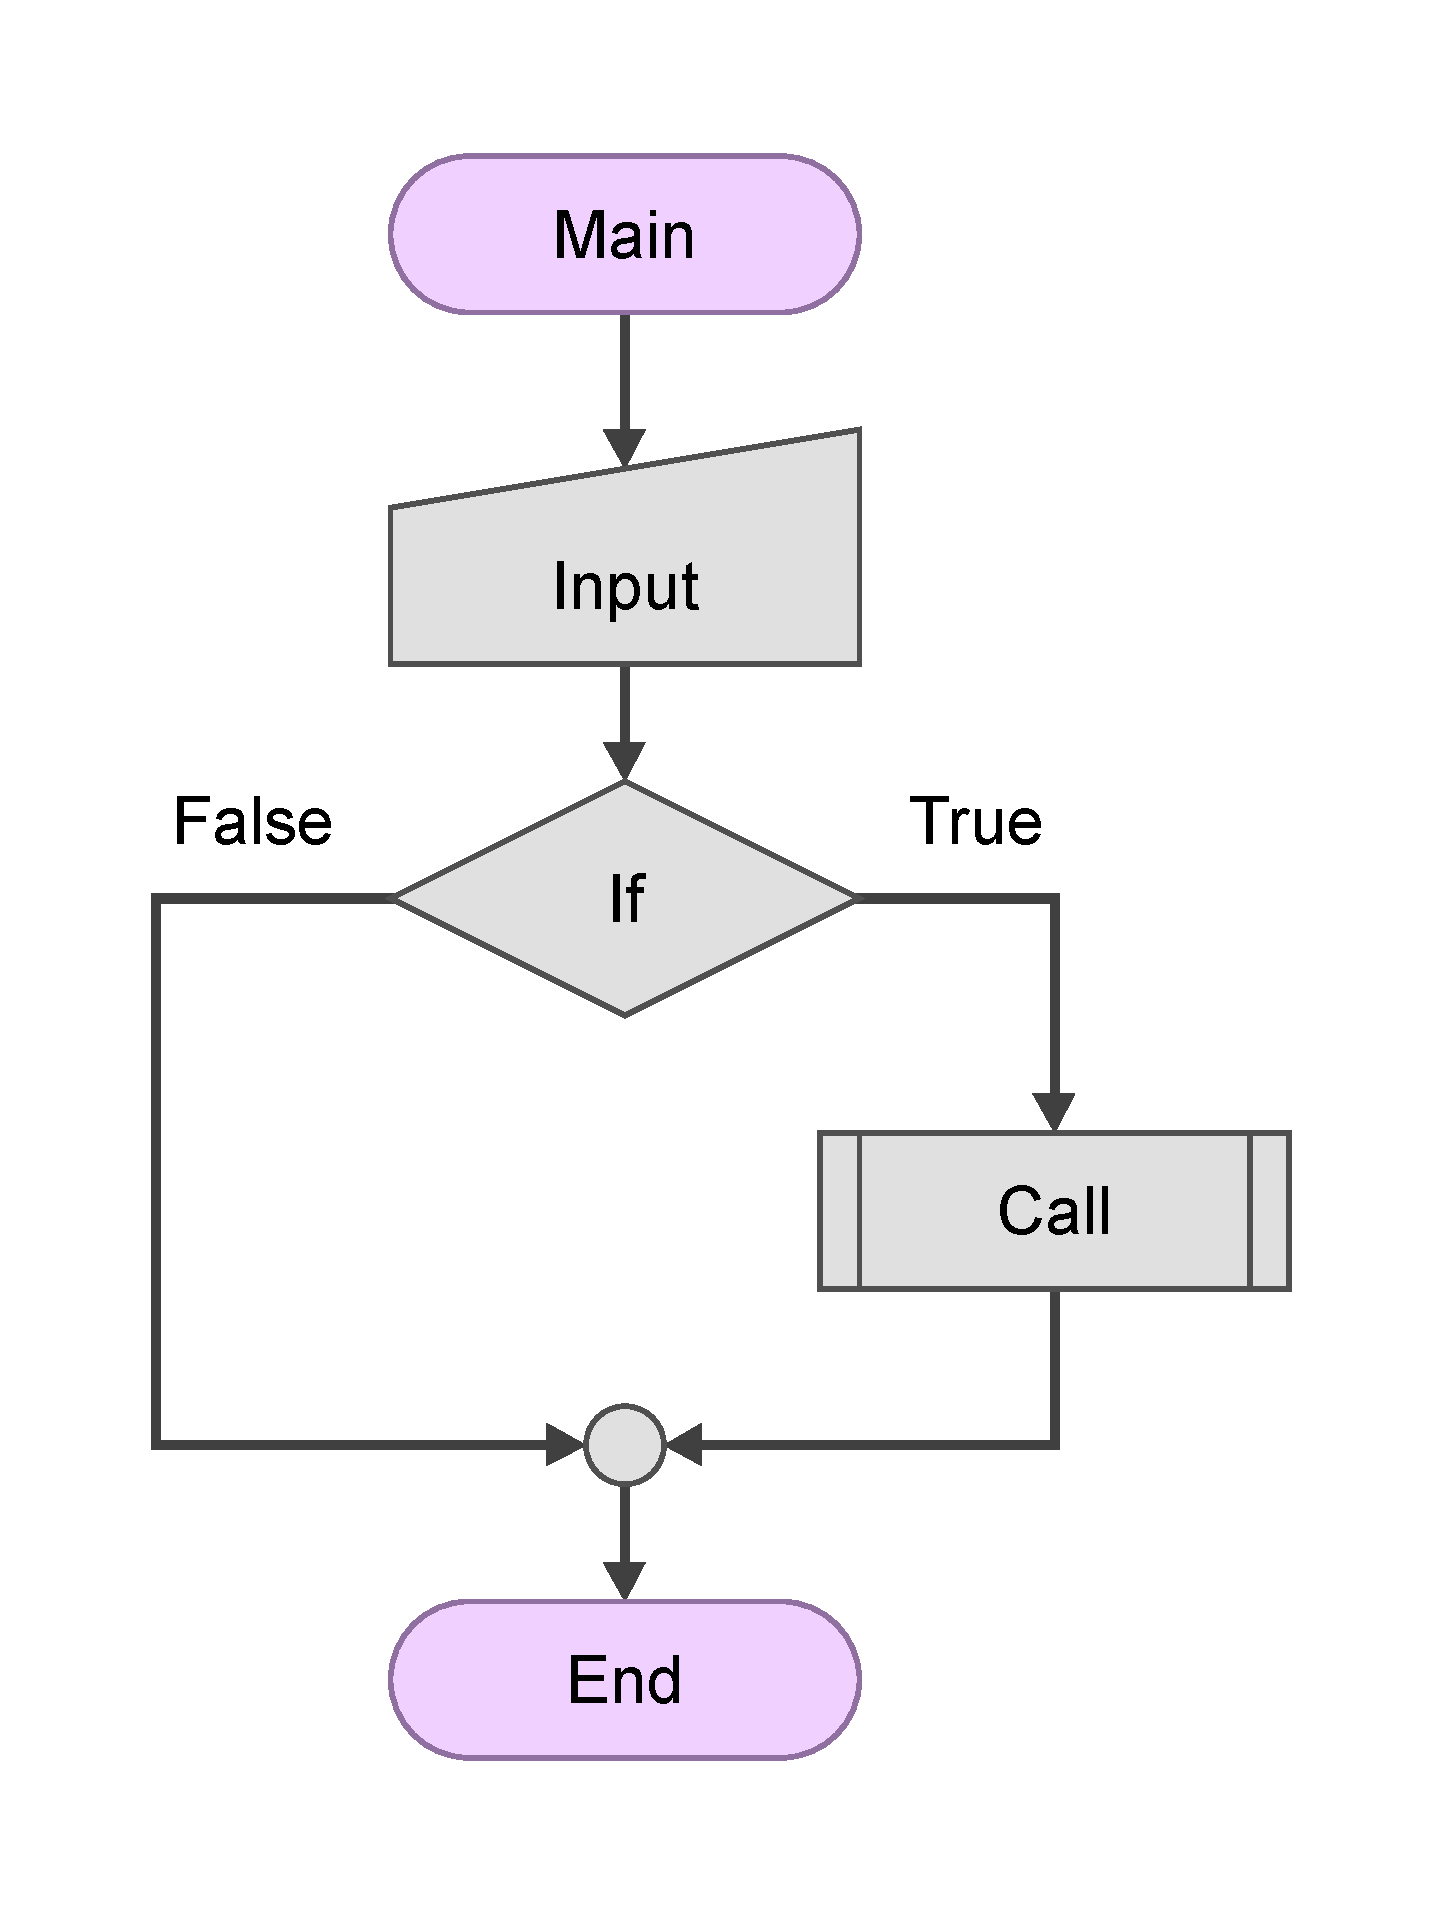
\includegraphics[scale=0.3]{figures/chart.pdf}
    \caption{Example figure in \LaTeX.}
    \label{fig:chart_a}
\end{figure}

\clearpage %  use command \clearpage when you want section or text to appear in the next page.

\section{Example of an algorithm in \LaTeX}
Algorithm~\ref{algo:algo_example} is a good example of an algorithm in \LaTeX.  
\begin{algorithm}
    \caption{Example caption: sum of all even numbers}
    \label{algo:algo_example}
    \begin{algorithmic}[1]
        \Require{$ \mathbf{x}  = x_1, x_2, \ldots, x_N$}
        \Ensure{$EvenSum$ (Sum of even numbers in $ \mathbf{x} $)}
        \Statex
        \Function{EvenSummation}{$\mathbf{x}$}
        \State {$EvenSum$ $\gets$ {$0$}}
        \State {$N$ $\gets$ {$length(\mathbf{x})$}}
        \For{$i \gets 1$ to $N$}                    
        \If{$ x_i\mod 2 == 0$}  \Comment check if a number is even?
        \State {$EvenSum$ $\gets$ {$EvenSum + x_i$}}
        \EndIf
        \EndFor
        \State \Return {$EvenSum$}
        \EndFunction
    \end{algorithmic}
\end{algorithm}
 
\section{Example of code snippet  in \LaTeX}

Code Listing~\ref{list:python_code_ex} is a good example of including a code snippet in a report. While using code snippets, take care of the following:
\begin{itemize}
    \item do not paste your entire code (implementation) or everything you have coded. Add code snippets only. 
    \item The algorithm shown in Algorithm~\ref{algo:algo_example} is usually preferred over code snippets in a technical/scientific report. 
    \item Make sure the entire code snippet or algorithm stays on a single page and does not overflow to another page(s).  
\end{itemize}

Here are three examples of code snippets for three different languages (Python, Java, and CPP) illustrated in Listings~\ref{list:python_code_ex}, \ref{list:java_code_ex}, and \ref{list:cpp_code_ex} respectively.  

\begin{lstlisting}[language=Python, caption={Code snippet in \LaTeX ~and  this is a Python code example}, label=list:python_code_ex]
import numpy as np

x  = [0, 1, 2, 3, 4, 5] # assign values to an array
evenSum = evenSummation(x) # call a function

def evenSummation(x):
    evenSum = 0
    n = len(x)
    for i in range(n):
        if np.mod(x[i],2) == 0: # check if a number is even?
            evenSum = evenSum + x[i]
    return evenSum
\end{lstlisting}

Here we used  the ``\textbackslash clearpage'' command and forced-out the second listing example onto the next page. 
\clearpage  %
\begin{lstlisting}[language=Java, caption={Code snippet in \LaTeX ~and  this is a Java code example}, label=list:java_code_ex]
public class EvenSum{ 
    public static int evenSummation(int[] x){
        int evenSum = 0;
        int n = x.length;
        for(int i = 0; i < n; i++){
            if(x[i]%2 == 0){ // check if a number is even?
                evenSum = evenSum + x[i];
            }
        }
        return evenSum;     
    }
    public static void main(String[] args){ 
        int[] x  = {0, 1, 2, 3, 4, 5}; // assign values to an array
        int evenSum = evenSummation(x);
        System.out.println(evenSum);
    } 
} 
\end{lstlisting}


\begin{lstlisting}[language=C, caption={Code snippet in \LaTeX ~and  this is a C/C++ code example}, label=list:cpp_code_ex]
int evenSummation(int x[]){
    int evenSum = 0;
    int n = sizeof(x);
    for(int i = 0; i < n; i++){
        if(x[i]%2 == 0){ // check if a number is even?
            evenSum = evenSum + x[i];
    	}
    }
    return evenSum;     
}

int main(){
    int x[]  = {0, 1, 2, 3, 4, 5}; // assign values to an array
    int evenSum = evenSummation(x);
    cout<<evenSum;
    return 0;
}
\end{lstlisting}



\section{Example of in-text citation style}
\subsection{Example of the equations and illustrations placement and reference in the text}
Make sure whenever you refer to the equations, tables, figures, algorithms,  and listings for the first time, they also appear (placed) somewhere on the same page or in the following page(s). Always make sure to refer to the equations, tables and figures used in the report. Do not leave them without an \textbf{in-text citation}. You can refer to equations, tables and figures more them once.

\subsection{Example of the equations and illustrations style}
Write \textbf{Eq.} with an uppercase ``Eq`` for an equation before using an equation number with (\textbackslash eqref\{.\}). Use ``Table'' to refer to a table, ``Figure'' to refer to a figure, ``Algorithm'' to refer to an algorithm and ``Listing'' to refer to listings (code snippets). Note that, we do not use the articles ``a,'' ``an,'' and ``the'' before the words Eq., Figure, Table, and Listing, but you may use an article for referring the words figure, table, etc. in general.

For example, the sentence ``A report structure is shown in \textbf{the} Table~\ref{tab:gen_template}'' should be written as ``A report structure is shown \textbf{in} Table~\ref{tab:gen_template}.'' 
 

\section{Summary}
Write a summary of this chapter.

~\\[5em]
\noindent
{\huge\textbf{Note:}} In the case of \textbf{software engineering} project a Chapter ``\textbf{Testing and Validation}'' should precede the ``Results'' chapter. See Section~\ref{subsec:se_chpters} for report organization of such project. 


    \chapter{Results}

\section{Results for CNN}
\label{ch:results}
Evaluating the performance of a Convolutional Neural Network (CNN) subjected to varying levels of Gaussian noise, using accuracy as the primary metric. The analysis uses three datasets: training, validation, and testing, to observe how the CNN copes with noise during different phases of model usage.

\begin{figure}[htbp]
  \centering
  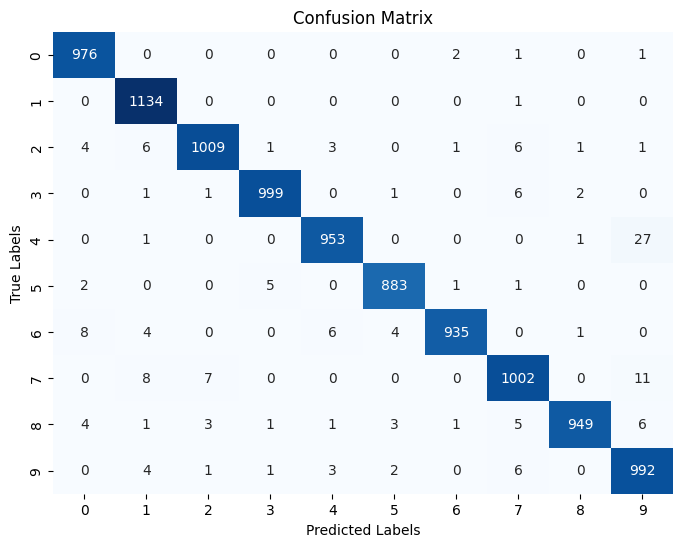
\includegraphics[width=0.7\textwidth]{figures/NL5_Confusionmatrix.png}
  \caption{Confusion Matrix for Noise level 0.5}
  \label{fig:nl5_cm}
\end{figure}


\begin{figure}[htbp]
  \centering
  \begin{minipage}{0.49\textwidth}
    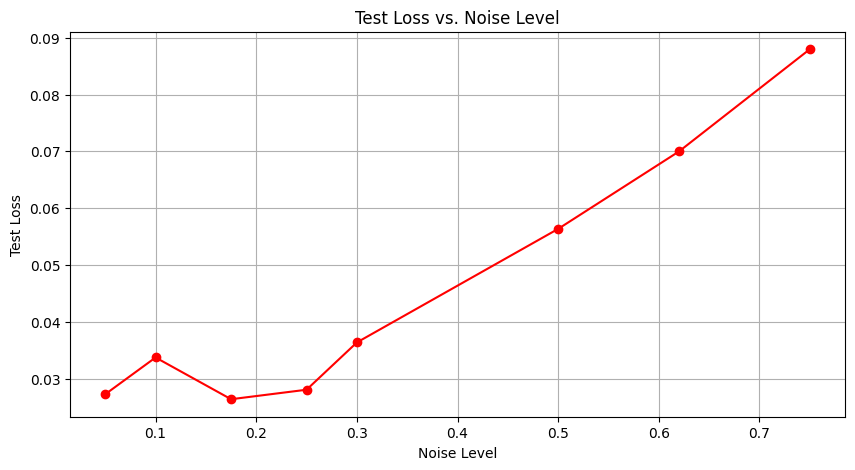
\includegraphics[width=\linewidth]{figures/cnn_testloss.png}
    \caption{CNN Test Loss}
    \label{fig:cnn_testloss}
  \end{minipage}\hfill
  \begin{minipage}{0.49\textwidth}
    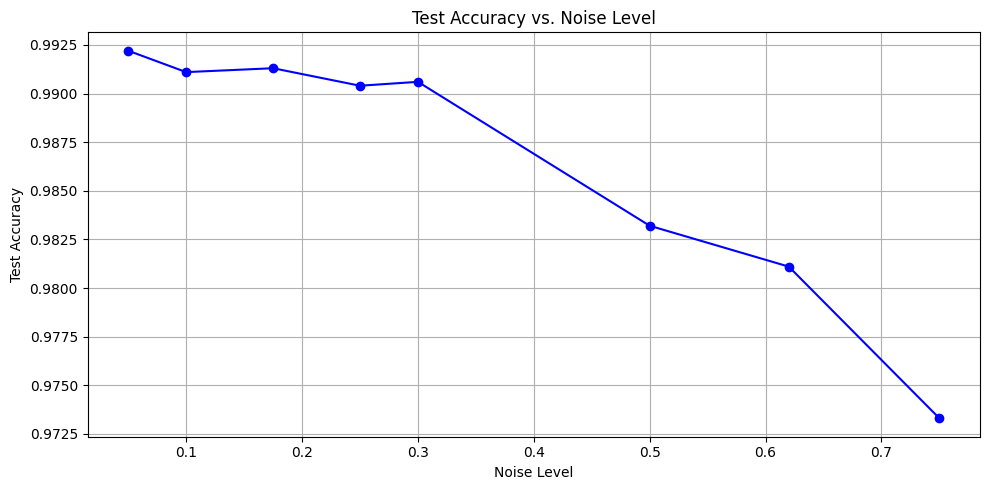
\includegraphics[width=\linewidth]{figures/cnn_testaccuracy.png}
    \caption{CNN Test Accuracy}
    \label{fig:cnn_testaccuracy}
  \end{minipage}
\end{figure}


\begin{table}[h!]
    \centering
    
    \begin{tabular}{|c|c|c|c|c|c|c|c|c|}
        \hline
        \multirow{2}{*}{CNN} & \multicolumn{8}{c|}{Noise Level} \\ \cline{2-9}
                             & 0.05 & 0.1 & 0.175 & 0.25 & 0.3 & 0.5 & 0.62 & 0.75 \\ \hline
        Training              & 99.56\% & 99.55\%  & 99.65\%  & 99.42\%  & 99.18\%  & 98.35\%  & 97.17\%  & 93.88\%  \\ \hline
        Validation            & 98.65\% & 98.77\% & 99.02\%  & 98.07\% & 98.08\% & 96.28\% & 94.46\% & 89.99\% \\ \hline
        Testing               & 98.99\% & 99.07\% & 98.98\%  & 98.91\% & 98.84\% & 98.54\% & 98.46\% & 97.74\% \\ \hline
    \end{tabular}
    \caption{CNN Accuracy Across Different Noise Levels}
\end{table}

The testing accuracy starts at a high of 98.99\% with minimal noise and remains robust up to a noise level of 0.5.



\section{Results for DAE}
The performance of a Denoising Autoencoder (DAE) when exposed to varying levels of Gaussian noise, evaluating its efficiency using reconstruction mean squared error (MSE) for assessing the quality of image reconstruction and training and validation losses to gauge model learning performance.

\begin{figure}[htbp]
  \centering
  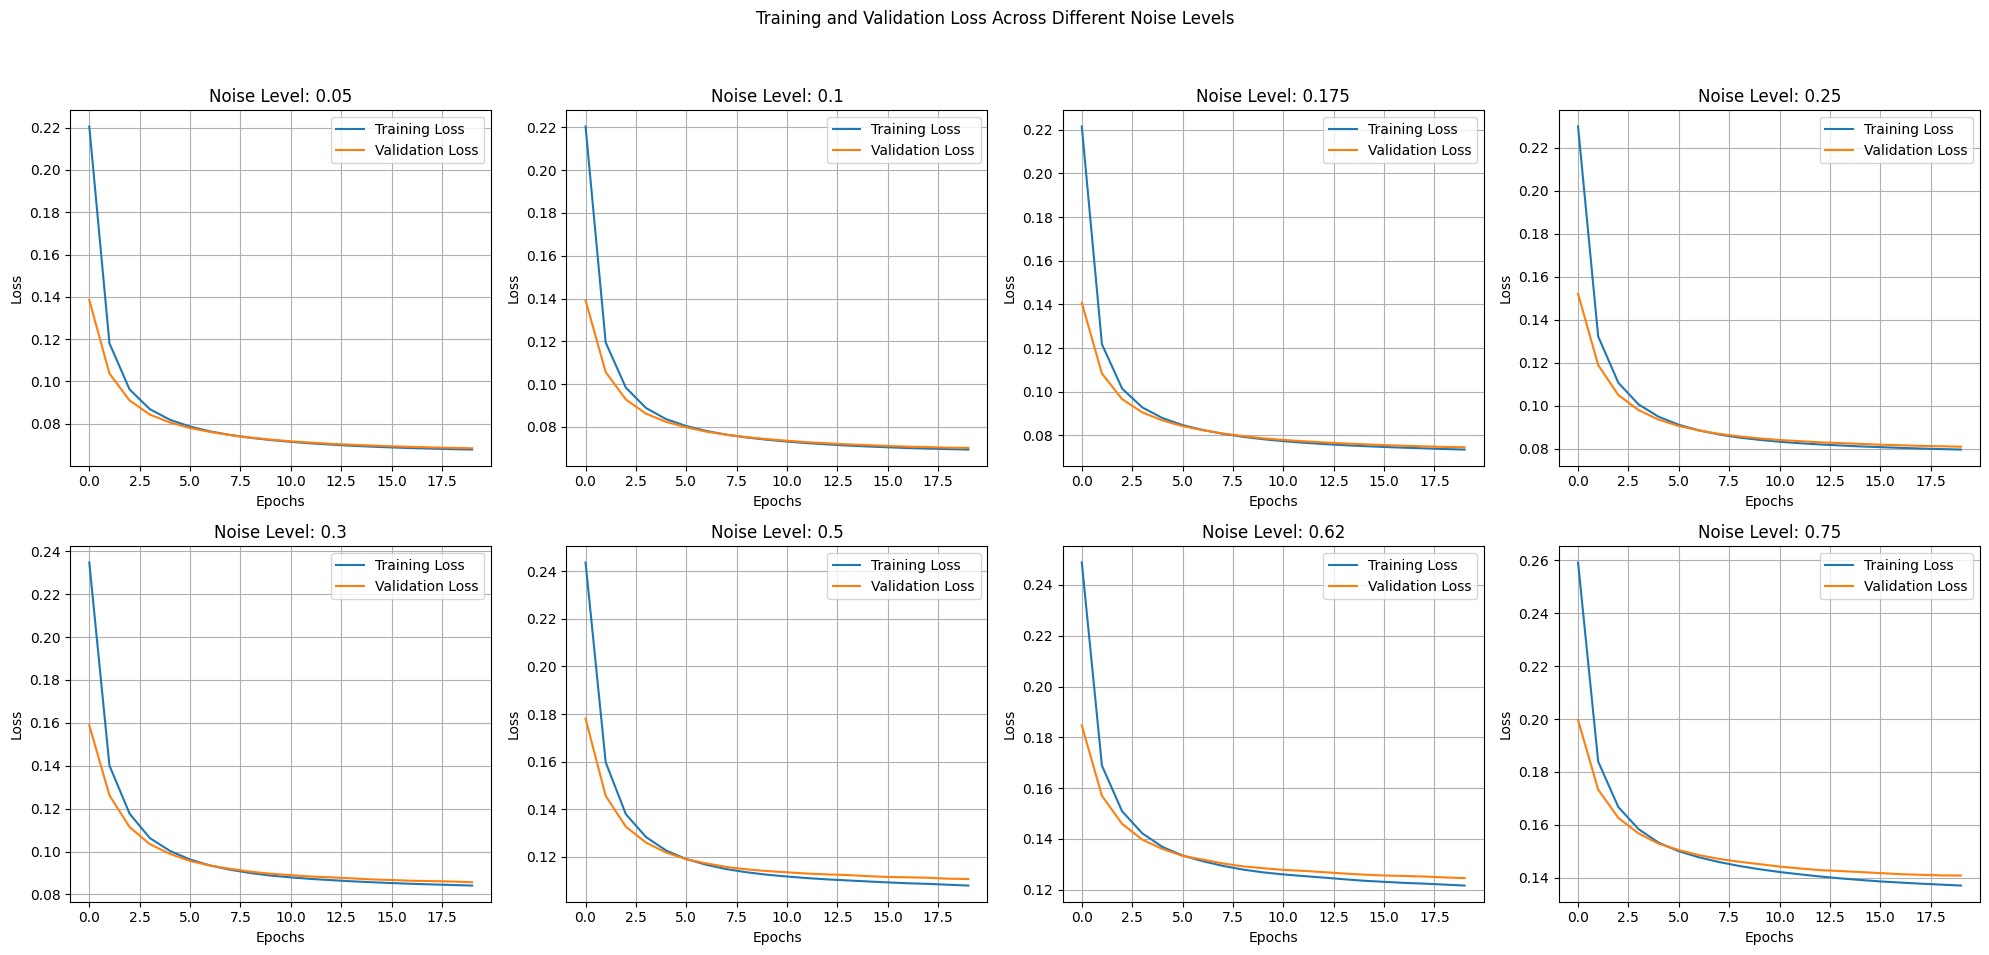
\includegraphics[width=0.8\textwidth]{figures/dae_TVloss.png}
  \caption{Training \& Validation Loss on various noise levels}
  \label{fig:dae_tvloss}
\end{figure}


\begin{figure}[htbp]
  \centering
  \begin{minipage}{0.49\textwidth}
    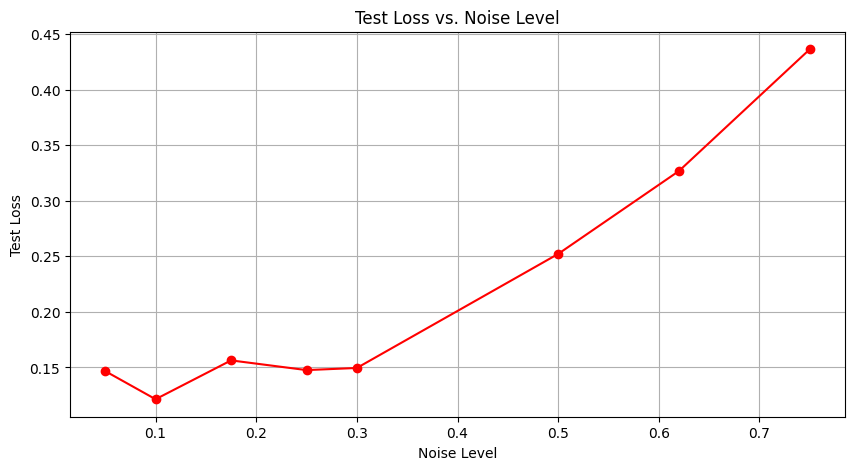
\includegraphics[width=\linewidth]{figures/dae_testloss.png}
    \caption{DAE Classifier Test Loss}
    \label{fig:dae_testloss}
  \end{minipage}\hfill
  \begin{minipage}{0.49\textwidth}
    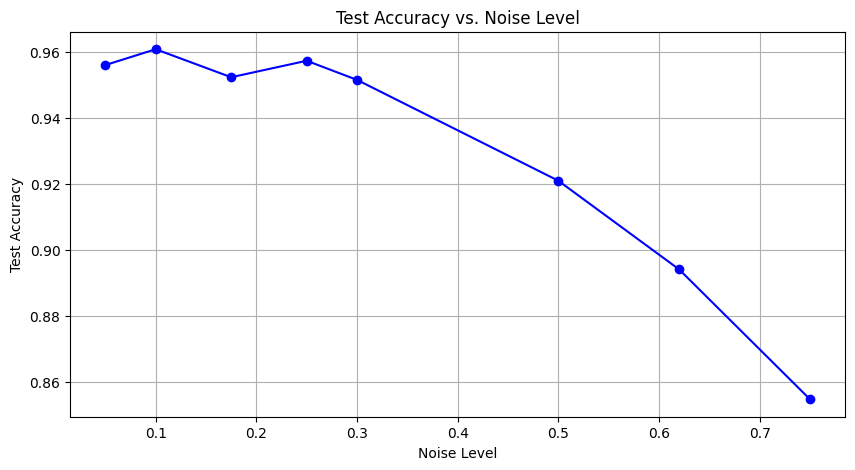
\includegraphics[width=\linewidth]{figures/dae_testaccuracy.png}
    \caption{DAE Classifier Test Accuracy}
    \label{fig:dae_testaccuracy}
  \end{minipage}
\end{figure}

\vspace*{1.2in}

\begin{table}[ht]
\centering
\label{tab:dae_performance}
\begin{tabular}{c|c|c|c}
\toprule
\textbf{Noise Level} & \textbf{Reconstruction MSE} & \textbf{Training Loss} & \textbf{Validation Loss} \\
\midrule
0.05 & 0.0021 & 0.0678 & 0.0684 \\
0.10 & 0.0026 & 0.0695 & 0.0702 \\
0.175 & 0.0038 & 0.0735 & 0.0746 \\
0.25 & 0.0057 & 0.0796 & 0.0809 \\
0.30 & 0.0072 & 0.0841 & 0.0857 \\
0.50 & 0.0148 & 0.1079 & 0.1106 \\
0.62 & 0.0195 & 0.1216 & 0.1245 \\
0.75 & 0.0249 & 0.1386 & 0.1418 \\
\bottomrule
\end{tabular}
\caption{Performance of Denoising Autoencoder (DAE) at Different Noise Levels}
\end{table}

\begin{figure}[htbp]
  \centering
  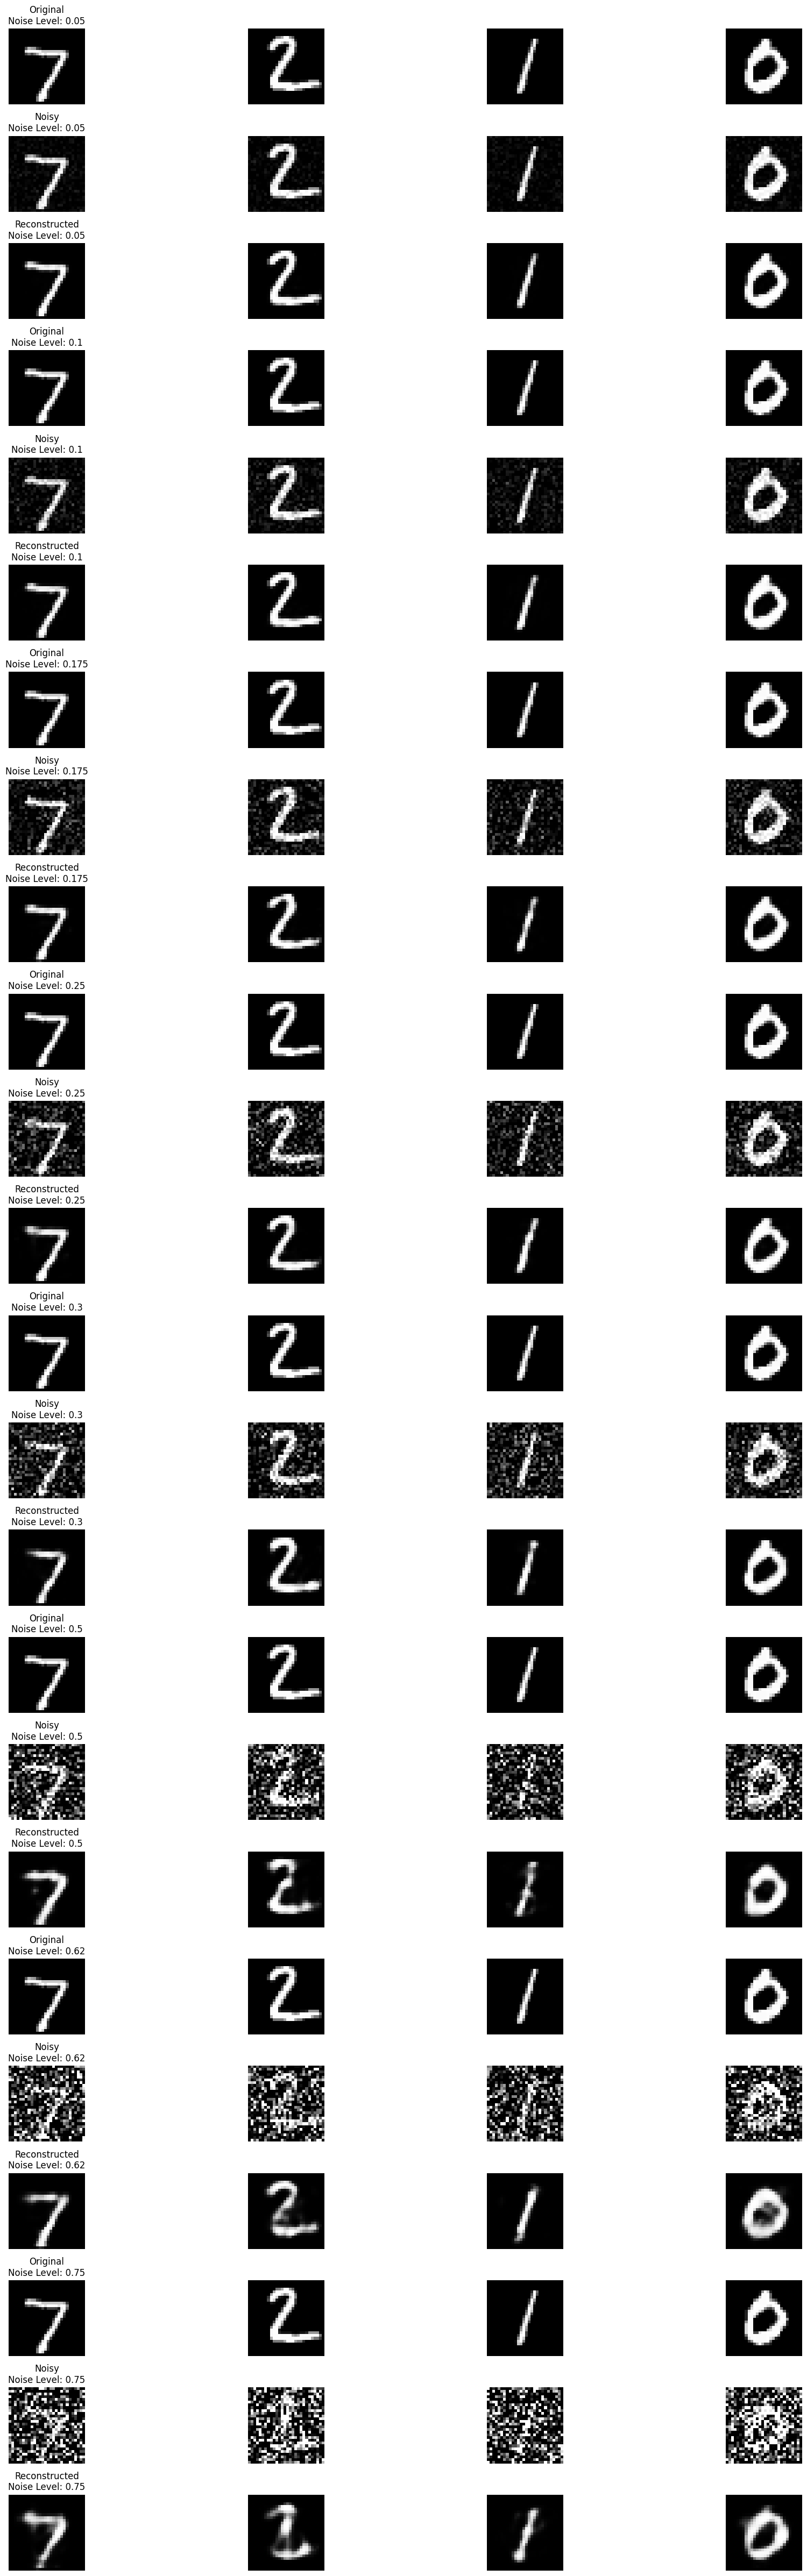
\includegraphics[width=0.8\textwidth]{figures/reconstructed_images.png}
  \caption{DAE Image Reconstruction on various noise levels}
  \label{fig:dae_imgreconst}
\end{figure}

\subsubsection{Image Reconstruction using DAE}
The image showcases a Denoising Autoencoder's (DAE) performance in cleaning digit images across a spectrum of Gaussian noise intensities. The format is arranged in a descending order of noise levels, with original images at the top, followed by noisy versions, and concluding with the DAE's reconstructed outputs at the bottom of each set. At lower noise levels, the DAE effectively restores the digits to a state closely resembling the originals. However, as noise intensifies, the quality of reconstruction degrades, revealing the DAE's decreasing ability to accurately denoise the images, especially when the noise reaches the highest levels. This visual demonstration effectively highlights the DAE's strengths in mitigating noise and its challenges in handling extreme noise conditions.



As shown in \ref{tab:dae_classifier_accuracy}  table presents the classification test accuracy of a Denoising Autoencoder (DAE) classifier at various noise levels, illustrating how the DAE's performance is affected as the noise level increases. Initially, at low noise levels (0.05 to 0.30), the DAE maintains high accuracy, slightly fluctuating but staying above 95\%. This indicates the DAE's strong capability to accurately classify images with minimal to moderate noise. However, as the noise level rises to 0.50 and beyond, there is a clear downward trend in accuracy, with a notable drop to 85.47\% at a noise level of 0.75. These figures underscore the challenge that higher noise levels pose to the DAE's classification ability, highlighting a decrease in performance as the noise approaches higher intensities.

\begin{table}[ht]
\centering
\begin{tabular}{c|c}
\toprule
\textbf{Noise Level} & \textbf{Accuracy (\%)} \\
\midrule
0.05 & 95.60\% \\
0.10 & 96.09\% \\
0.175 & 95.24\% \\
0.25 & 95.74\% \\
0.30 & 95.16\% \\
0.50 & 92.10\% \\
0.62 & 89.41\% \\
0.75 & 85.47\% \\
\bottomrule
\end{tabular}
\caption{Classification Test Accuracy of DAE Classifier at Various Noise Levels}
\label{tab:dae_classifier_accuracy}
\end{table}

\section{Summary}
The robustness and adaptability of both the Convolutional Neural Network (CNN) and the Denoising Autoencoder (DAE) when challenged by varying levels of Gaussian noise. The CNN maintains high accuracy across training, validation, and testing phases with minimal degradation until noise levels reach 0.5, demonstrating effective noise resilience. Conversely, the DAE, assessed through reconstruction MSE and training/validation losses, shows a gradual increase in error as noise levels rise, indicating a decline in its ability to reconstruct images precisely at higher noise intensities. Additionally, the classification accuracy of a DAE-based classifier also declines as noise increases, further illustrating the challenges faced by DAEs in maintaining performance under severe noise conditions. Together, these results highlight the strengths and limitations of both models in noise-affected environments, guiding potential improvements for noise robustness in neural network applications.




    \chapter{Discussion and Analysis}
\label{ch:evaluation}

\section{Discussion on performance on noise levels}
The performance of the Convolutional Neural Network (CNN) and the Denoising Autoencoder (DAE) across various Gaussian noise intensities reveals important insights into their operational resilience and constraints. The CNN showed commendable performance in maintaining high accuracy levels until a moderate noise intensity (0.5), beyond which a significant drop in accuracy was observed. This indicates that CNNs, with appropriate training, can efficiently process data in environments with considerable noise, which is essential for applications such as real-time surveillance or autonomous vehicle navigation.

On the other hand, the DAE demonstrated excellent initial performance in reducing noise at lower levels, as evidenced by low reconstruction MSE scores. However, as the noise intensity escalated, the effectiveness of the DAE diminished markedly, highlighted by rising MSE values. This decline might reflect the model's limitations in adapting to more complex or intense noise patterns, or a saturation in its data modeling capabilities.

\section{Significance of the findings}
The significance of these findings is underscored by demonstrating how various neural network architectures navigate the challenge of environmental noise, a prevalent issue in processing real-world data. Notably, the CNN's ability to sustain high accuracy up to moderate noise levels illustrates its suitability for critical applications such as autonomous vehicle navigation, where real-time image processing is essential and environmental conditions are unpredictable. This resilience suggests that CNNs could serve as a cornerstone technology for systems that demand consistent reliability across diverse sensory inputs.

For the Denoising Autoencoder (DAE), the notable reduction in reconstruction errors at lower noise intensities confirms its utility in enhancing image quality, critical for tasks such as digital photo restoration or improving the clarity of medical images, where precision is vital for accurate diagnosis. Additionally, the DAE’s ability to improve image quality before further analytical processing can lead to more precise outcomes in subsequent image-processing tasks like object detection or classification.

\section{Limitations} 
Despite the promising results, several limitations must be acknowledged, which could impact the generalizability and scalability of the findings:


\begin{itemize}
    \item Noise Diversity: The study's focus on Gaussian noise does not fully encapsulate the complexity of real-world scenarios, which often involve a variety of noise types including Poisson, speckle, and motion blur. This limitation underscores the need to test these models against a broader spectrum of noise conditions to ensure their robustness across different environments.

    \item Model Scalability: The increasing reconstruction MSE observed in the DAE as noise levels rise suggests potential scalability issues under extreme noisy conditions. This could limit the DAE's applicability in environments where noise is not only high but also diverse in nature, potentially impacting the model’s effectiveness in broader applications.

    \item Overfitting Concerns: The CNN's consistent performance up to a certain noise threshold might mask underlying overfitting issues, where the model is potentially tuned to specific noise characteristics rather than capturing more generalized patterns. Such overfitting could undermine the model’s performance in new or varied operational settings where noise characteristics differ from the training data.

    \item Computational Efficiency: Both CNNs and DAEs, especially as the models increase in complexity to handle higher levels of noise, place significant demands on computational resources. This could pose challenges in deploying these models in resource-constrained environments, potentially limiting their usability in real-time applications or on edge devices.

\end{itemize}


\section{Summary}
The analysis of Convolutional Neural Networks (CNNs) and Denoising Autoencoders (DAEs) under varying levels of Gaussian noise revealed their respective strengths and limitations in noisy environments. CNNs maintained robust performance up to moderate noise levels, indicating their practical utility, but showed a performance drop at higher noise intensities. DAEs effectively reduced noise at lower levels but struggled with higher noise, pointing to scalability issues. Both models faced challenges including overfitting and computational efficiency, emphasizing the need for further research to enhance their adaptability and efficiency in diverse real-world settings.
    \chapter{Conclusions and Future Work}
\label{ch:con}
\section{Conclusions}
Typically a conclusions chapter first summarizes the investigated problem and its aims and objectives. It summaries the critical/significant/major findings/results about the aims and objectives that have been obtained by applying the key methods/implementations/experiment set-ups. A conclusions chapter draws a picture/outline of your project's central and the most signification contributions and achievements. 

A good conclusions summary could be approximately 300--500 words long, but this is just a recommendation.

A conclusions chapter followed by an abstract is the last things you write in your project report.

\section{Future work}
This section should refer to Chapter~\ref{ch:results} where the author has reflected their criticality about their own solution. The future work is then sensibly proposed in this section.

\textbf{Guidance on writing future work:} While working on a project, you gain experience and learn the potential of your project and its future works. Discuss the future work of the project in technical terms. This has to be based on what has not been yet achieved in comparison to what you had initially planned and what you have learned from the project. Describe to a reader what future work(s) can be started from the things you have completed. This includes identifying what has not been achieved and what could be achieved. 



A good future work summary could be approximately 300--500 words long, but this is just a recommendation.
    \chapter{Reflection}
\label{ch:reflection}
%%%%%%%%%%%%%%%%%%%%%%%%%%%%%%%
%% Please remove/replace text below
%%%%%%%%%%%%%%%%%%%%%%%%%%%%%%%
Write a short paragraph on the substantial learning experience. This can include your decision-making approach in problem-solving.

\textbf{Some hints:} You obviously learned how to use different programming languages, write reports in \LaTeX and use other technical tools. In this section, we are more interested in what you thought about the experience. Take some time to think and reflect on your individual project as an experience, rather than just a list of technical skills and knowledge. You may describe things you have learned from the research approach and strategy, the process of identifying and solving a problem, the process research inquiry, and the understanding of the impact of the project on your learning experience and future work.

Also think in terms of:
\begin{itemize}
    \item what knowledge and skills you have developed
    \item what challenges you faced, but was not able to overcome
    \item what you could do this project differently if the same or similar problem would come
    \item rationalize the divisions from your initial planed aims and objectives.
\end{itemize}


A good reflective summary could be approximately 300--500 words long, but this is just a recommendation.

~\\[2em]
\noindent
{\huge \textbf{Note:}} The next chapter is ``\textbf{References},'' which will be automatically generated if you are using BibTeX referencing method. This template uses BibTeX referencing.  Also, note that there is difference between ``References'' and ``Bibliography.'' The list of ``References'' strictly only contain the list of articles, paper, and content you have cited (i.e., refereed) in the report. Whereas Bibliography is a list that contains the list of articles, paper, and content you have cited in the report plus the list of articles, paper, and content you have read in order to gain knowledge from. We recommend to use only the list of ``References.'' 

    

    
    % -------------------------------------------------------------------
    % Bibliography/References  -  Harvard Style was used in this report
    % -------------------------------------------------------------------
    \bibliographystyle{agsm} % Harvard Style 
    
    \bibliography{references}  %  Patashnik, O. (1988), BibTEXing. Documentation for general BibTEX users.
    
    % -------------------------------------------------------------------
    % Appendices
    % -------------------------------------------------------------------
    
    \begin{appendices}
        \chapter{An Appendix Chapter (Optional)}
\label{appn:A}
% Optional chapter
Some lengthy tables, codes, raw data, length proofs, etc. which are \textbf{very important but not essential part} of the project report goes into an Appendix. An appendix is something a reader would consult if he/she needs extra information and a more comprehensive understating of the report. Also, note that you should use one appendix for one idea.

An appendix is optional. If you feel you do not need to include an appendix in your report, avoid including it. Sometime including irrelevant and unnecessary materials in the Appendices may unreasonably increase the total number of pages in your report and distract the reader.


        \chapter{An Appendix Chapter (Optional)}
\label{appn:B}

...
    \end{appendices}
    
\end{document}
